\section{Method}
\label{sec:method}

% WRITING PROMPTS (comments only; they do not print). About 3 pages. The
% reference draft is notes/method-draft.tex (equations, GA and PSO settings);
% note it predates sweep angles per cell: variants are now 4 sweep angles
% (0, 45, 90, 135 deg) x 4 start corners.
%
% Walk the reader through Fig. pipeline, one subsection per panel:
%  (a) free area: the lawn eroded by c = w/2;
%  (b) boustrophedon cells along the lane direction;
%  (c) back-and-forth lanes in each cell, m = ceil(b/w) lanes;
%  (d) A* on the visibility graph between cells, and the visiting order.
% Then the transition table and the exact variant DP (Eq. variant-dp).
%
% Decomposition direction (new since the draft; see the README section
% "Our method: energy-chosen decomposition direction"). Explain with Fig.
% direction-choice: candidates are the headings of the lawn's edges (Huang
% 2001), each is scored by a 500-evaluation GA run, and the least-energy one
% is kept. On the garden lawn the chosen 0 deg heading needs 15.3 kJ against
% 17.0 kJ for the default 90 deg. Say that the choice is paid from the same
% 20 000-evaluation budget.
%
% Cell ordering: GA (main) and PSO (variant), parameters in the draft.
%
% Path tracking on the robot (short subsection): stop-turn-go, as the planner
% costs it. The fuzzy steering controller (Fig. fuzzy-controller): five
% triangular sets on the cross-track and heading errors, 25 Sugeno rules with
% constant outputs, steering against the sum of both errors. Say how the
% yaw-rate gain is learned from the gyro (tracker.py, YawGain).
%
% Question to settle: does the PSO earn its place in the paper? If you keep
% it, say why in one sentence (a second soft-computing search confirms that
% the gain comes from the objective, not from the GA).

\begin{figure*}[t]
\centering
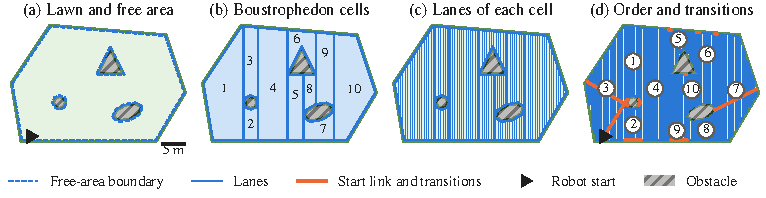
\includegraphics[width=\textwidth]{pipeline}
% DRAFT caption: rewrite in your own words.
\caption{Planning pipeline on the \texttt{garden} lawn. (a) The free area keeps the robot centre half a cutting width from every edge. (b) Boustrophedon cells. (c) Back-and-forth lanes of each cell. (d) The plan: the visiting order of the cells and the A* transitions between them.}
\label{fig:pipeline}
\end{figure*}

\begin{figure*}[t]
\centering
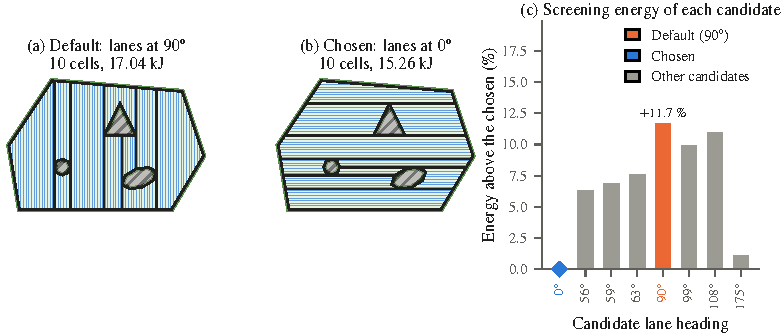
\includegraphics[width=\textwidth]{direction-choice}
% DRAFT caption: rewrite in your own words.
\caption{Choice of the decomposition direction on the \texttt{garden} lawn. (a) Default direction. (b) Direction chosen by energy. (c) Energy of a short GA run for each candidate heading, parallel to an edge of the lawn or of an obstacle, above that of the chosen heading (diamond).}
\label{fig:direction-choice}
\end{figure*}

\begin{figure*}[t]
\centering
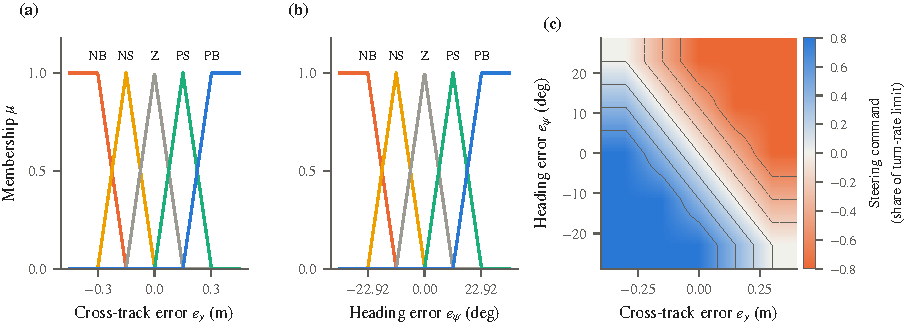
\includegraphics[width=\textwidth]{fuzzy-controller}
% DRAFT caption: rewrite in your own words.
\caption{Fuzzy steering controller of the path tracker. Membership functions of (a) the cross-track error and (b) the heading error. (c) Steering command over both errors (zero-order Sugeno rules, weighted average).}
\label{fig:fuzzy-controller}
\end{figure*}
